\documentclass{article}
\usepackage[utf8]{inputenc}
\usepackage{enumitem}
\usepackage{nameref}
\usepackage{graphicx}

\title{Software Engineering 2 Project}
\author{Stefano Martina, Alessandro Nichelini, Francesco Peressini}

\begin{document}

\maketitle
\newpage

\tableofcontents
\newpage

\section{Introduction}

\subsection{Purpose}

TrackMe is a company aiming to support interactions between users, 
who like keeping track of the health status and their activities, and
third parties which can use data and enhance their value.

TrackMe app is composed of three main important service:
\begin{itemize}
\item Data4Help: basic support for health data;
\item AutomatedSOS: add support for SOS services to elderly people;
\item Track4Run: add support for running events.
\end{itemize}

Each of them will have as targets:
\begin{itemize}
\item Individuals users
\item Third parties.
\end{itemize}
Since each service serves both the targets, the project consists of 
platform divided in a mobile application and a web-based interface to
serve third-parties.

The system allows individual users to add and handle data on the app
and to third parties to request and have access to these data.

In particular, a user of the application is able to keep track of 
his/her position during the activities but also during the normal 
day-life. The users’ data are used to monitor the heartbeat and 
eventually to send an AutomatedSOS.
Furthermore, TrackMe, is able to track all the athletes (that are 
using the application), during a run previously organised. 
Indeed TrackMe’s app provide a section to setup a group run, 
specifying the path and other useful information.

\subsection{Scope}
\subsubsection{Description of the problem}
Nowadays a lot of persons track their activities with smartphone or
smartwatch. For this reason TrackMe provide a new complete user 
experience allowing all the user to read briefly all the information
about all activities’ history.
It’s also provided a service to organise a group run, during which
it’s possible to monitor all the athletes information.
Furthermore all the users are monitored and, in case of some trouble, 
an SOS will be launched.
\newpage
\subsubsection{World Phenomena}
\begin{itemize}
	\item \textit{General user’s health condition}: the machine doesn’t know the information about possible user’s disease.
	\item \textit{First aid services status}: the machine doesn’t know the actual first aid services status.
	\item \textit{Overall third parties knowledge status}: the machine doesn’t know which informations third parties already have about users.
\end{itemize}

\subsubsection{Machine Phenomena}
\begin{itemize}
	\item \textit{Third-parties registration};
	\item \textit{User's registration};
	\item \textit{Data anonymisation}.
\end{itemize}

\subsubsection{Shared Phenomena}
\begin{itemize}
	\item \textit{Vital parameters}: the machine can read vital parameters of the user such as BPM.
	\item \textit{User's location}: the machine knows or can read actual and past user’s location.
\end{itemize}

\subsubsection{Goals} \label{goals}
\begin{enumerate}[label={\textbf{[G\arabic*]}}]
\item Users can be recognised by their credentials.
\item Allow users to keep track of their health data.
\item Allow users to have access to an overview of their data, including health parameters and performed activities. \label{g3}
\item Allow users to manage their data access policy.
\item Allow users to monitor their performance during run workouts.
\item Each time vital signs go below a threshold value, first aid services have to be notified.
\item Allow users to organise running events.
		\begin{enumerate}[label={[G\arabic{enumi}.\arabic*]}]
    		\item Allow users to create running events.
    		\item Allow users to en-roll to events.
    		\item Allow spectators to follow participants’ live position during events.
  		\end{enumerate}
\item Allow third parties to access data:
		\begin{enumerate}[label={[G\arabic{enumi}.\arabic*]}]
    		\item Allow third parties to require access to specific user data.
    		\item Allow third parties to retrieve anonymised aggregated data.
    		\item Allow third parties to subscribe to da
  		\end{enumerate}

\end{enumerate}

\subsection{Definitions, Acronyms, Abbreviations}

\subsubsection{Definitions}
\begin{itemize}
	\item \textbf{Event:} An event organized by a user (\textit{ e.g scenario 3.6.3)}.
	\item \textbf{Notification:} A warning that advise the user of a request by third parties.
	\item \textbf{AGGIUNGERE ALTRO?} 
	\end{itemize}

\subsubsection{Acronyms}
\begin{itemize}
\item API: Application Programming Interface;
\item ASOS: AutomatedSOS;
\item BPM: Beats Per Minutes;
\item D4H: Data4Help;
\item RASD: Requirement Analysis and Specification Document;
\item T4R: Track4Run.
\end{itemize}

\subsubsection{Abbreviations}
\begin{itemize}
		\item \begin{math}[Gn]\end{math}: n-th goal
		\item \begin{math}[Dn]\end{math}: n-th domain assumption 
		\item \begin{math}[Rn]\end{math}: n-th functional requirement
\end{itemize}

\subsection{Revision history}
\begin{itemize}
	\item 1.0.0 Initial version (10-11-2018)
\end{itemize}
\subsection{Reference Documents}
\subsection{Document Structure}
\newpage
\section{Overall description}

\subsection{Product perspective}
\subsubsection{Class Diagram}
The product perspective of TrackMe is now explained using the UML paradigms.
The main classes of the UML are:
\begin{itemize}
	\item \textbf{User} contains all the information about a user like username, password, fiscalCode, hometown, elderly, runners.
	\item \textbf{ThirdParties} contains all the information about the registered organisation.
	\item \textbf{Data} is an abstract class that has two concrete classes: 
		\textbf{Health data} and	 \textbf{Location data}
	\item \textbf{Running Event} 
	\item \textbf{Location} contains information like the start point and the end point of a running event.
\end{itemize}

A user creates an Event specifying the path ie the starting location, the ending location and some specific interesting point along the path.
After the creation some user can join in.
An organisation, as explained above, can subscribe to a feed of data or directly to a single user.


\begin{figure}[h!]
  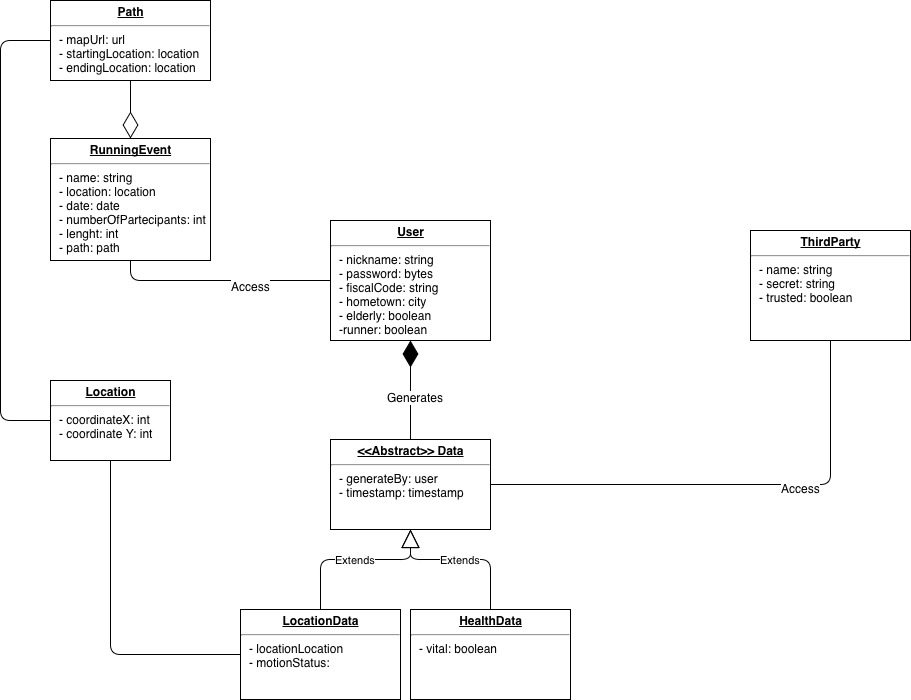
\includegraphics[width=\textwidth]{Figures/ClassDiagram.jpg}
  \caption{UML diagrams.}
  \label{fig:umlDiagrams}
\end{figure}
\newpage

\subsubsection{State Diagram}
The whole system can be also seen as a set of different services relying on the main module Data4Help.
Here we describe the main aspects of them with state diagrams.

\begin{figure}[h!]
  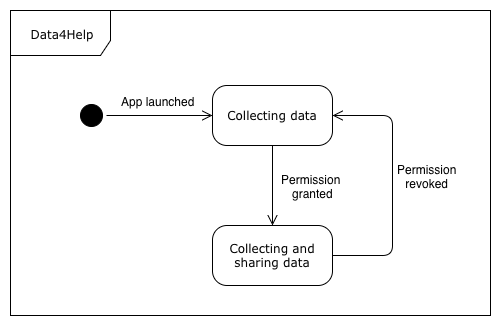
\includegraphics[width=\textwidth]{Figures/State1}
  \caption{Basic Data4Help service state diagram.}
  \label{fig:State1}
  
  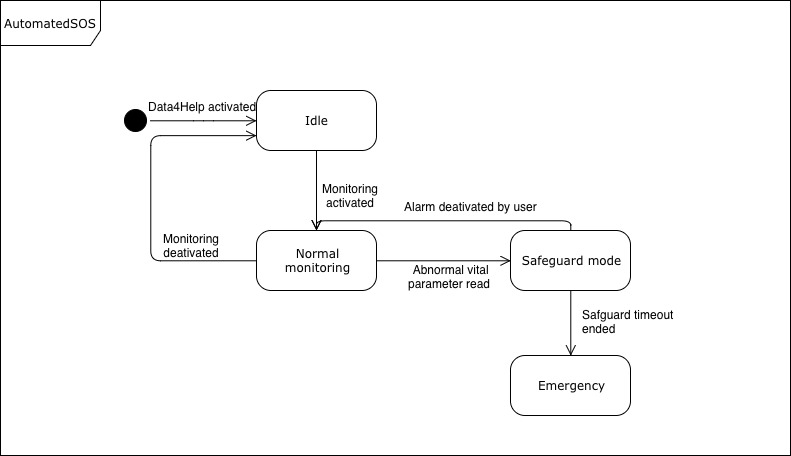
\includegraphics[width=\textwidth]{Figures/State2}
  \caption{Automated SOS state diagram.}
  \label{fig:State2}
\end{figure}

\newpage
	
\begin{figure}[h!]
  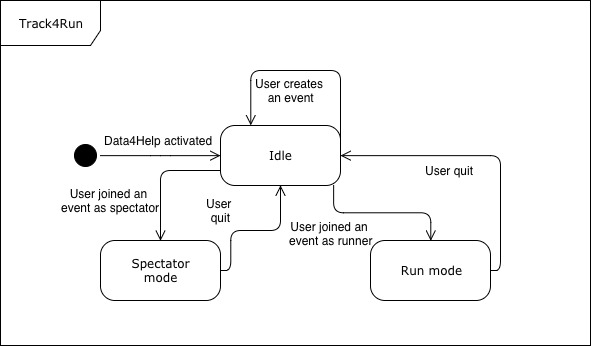
\includegraphics[width=\textwidth]{Figures/State3}
  \caption{Track4Run state diagram}
  \label{fig:State3.}
\end{figure}

\subsection{Product functions}
The software developed by TrackMe included three different services:
Data4Help supports user's data acquiring through smartwatches or 
similar devices, AutomatedSOS, a personalised and non-intrusive SOS 
service for elderly people and Track4Run, a service to track athletes 
participating to a run.
Data4Help is also a service available for third-parties: in fact, 
organisations can request data to TrackMe and collect them for 
pursuing their objectives.
Data acquisition can be performed in two different way: directly to a
single user or to a groups of individuals.
Concerning the single user case, companies, through a social security
code, ask permission to access the corresponding information. 
In the other case, organisations can request, directly to TrackMe,
data of group of individuals with particular proprieties (e.g. users 
between 20 and 30 years old or living in a certain district).
In the latter, TrackMe provides data only if it can anonymised them
correctly.
AutomatedSOS it’s great for those elderly people who want to monitor 
their health status and have the support of an ambulance in case their
vital parameters are under certain thresholds.
Track4Run it’s a service dedicated to the runners: it offers the 
possibility to organise a run between other runners, define the path 
and the duration, allowing the invited ones to en-roll. In addition, 
Track4Run users who do not partecipate to the run can see live time 
on a map the position of all the runners. 
Finally, Track4Run supports the synchronisation of data with 
Data4Help.

All the goals presented in section \ref{goals} are going to be 
implemented. Here we describe deeply the requirements needed to
implement application's functions.
	
\begin{enumerate}[label={[R\arabic*]}]
    	\item Users can create an account with credentials.
    	\item Credentials can be retrievable also if forgotten/lost.
    	\item Users can log manually or automatically their data.
    	\item Users have to be able to accept/deny access to single data access request.
    	\item Users have to be able to see current data policies and to change them.
    	\item The machine has to be able to read health and position data.
		\item The machine has to be able to recognise below threshold parameters.
		\item The machine has to be able to communicate with third parties.
		\item The machine has to be able to recognise data fragmentation level 
		\item The machine has to be able to store users’ data. 
\end{enumerate}

\subsection{Users characteristics}
\textbf{Users}: any person that will use the service to keep track of health data, positioning or automated SOS during any kind of activities (walking or running during a lone run or an organised event).\\\\
\textbf{Third parties}: Organisation or other parties interested in the acquisition for their usage of the data provided by the user activities.

\subsection{Assumptions, dependencies and constraints}

\subsubsection{Domain assumptions}

\begin{enumerate}[label={[D\arabic*]}]
    	\item Data manually logged by users well describes reality.
    	\item First aid services are ready to handle emergency notifications.
    	\item Data inserted by users are truthful 
    		\begin{enumerate}[label={[D\arabic{enumi}.\arabic*]}]
    			\item Data are up to date.
    			\item Data are correctly formatted.
  			\end{enumerate}
  		
  		\item Running paths proposed by users are well formed (e.g: legit by law).
  		\item External services are reliable.
\end{enumerate}

\newpage
\section{Specific Requirements}

\subsection{External Interface Requirements}

	\subsubsection{User Interfaces} 
	
	\subsubsection{Hardware Interfaces}
	The system requires one or more dedicated servers for data 
	management and for handling communication between users and 
	third-parties.
	
	\subsubsection{Software Interfaces}
	\begin{itemize}
		\item \textbf{Data4Help} \newline 
		User's health data can be inserted in Data4Help section of the
		application manually or automatically synchronised with data
		acquired by individual's wearable device with HealthKit API 
		provided by Apple. \newline
		Third-parties can access to the different data through a 
		web-based interface in which, in case the organisation is 
		interested to the information of some specific individual, 
		can select the single user by his/her fiscal code and send to
		him/her the request of data's visualisation; instead, in the 
		case of interest in accessing data of groups of individuals, 
		companies can select the parameters of interest and send to 
		TrackMe the request on hold for a positive response. \newline
		Data4Help also offers the integration with ResearchKit and 
		CareKit APIs, also provided by Apple, to help third-parties to 
		access more relevant data for their studies.
		\item \textbf{AutomatedSOS} \newline
		Similarly as Data4Help, AutomatedSOS automatically 
		synchronises data acquired from user's wearable device and 
		monitors them to guarantee the safety of elderly people. 
		\newline
		In case of emergency, an ambulance will reach the location
		of the costumer: AutomatedSOS uses Google Maps API to show 
		live-time the position on the map of the arriving ambulance. 
		\item \textbf{Track4Run} \newline
		Since Track4Run aims to schedule and organise runs for the 
		users of the service, it makes use of Google Calendar API to 
		allow individuals to create and en-roll races. 
		Also, for users not taking part of runs, Track4Run supports 
		Google Maps API for live-tracking the position of the 
		participating runners. 
	\end{itemize} 
	
	\subsubsection{Communication Interfaces}
\newpage
\subsection{Functional Requirements}	
	\subsubsection{Definitions of use cases}
	
\begin{table}[h!]
\centering
\begin{tabular}{|l|l|} 
\hline
Name             & Sing up                                                                                                                                                                                                                                                                                  \\ 
\hline
Actor            & User                                                                                                                                                                                                                                                                                     \\ 
\hline
Entry conditions & The application has been correctly installed on user's iOS device                                                                                                                                                                                                                        \\ 
\hline
Events flow      & \begin{tabular}[c]{@{}l@{}}1. Select the "Sing up" option~\\2. Fill in all the fields necessary for registering to the services~\\3. Confirm your inputed data\end{tabular}                                                                                                             \\ 
\hline
Exit conditions  & \begin{tabular}[c]{@{}l@{}}Data has been successfully saved and the costumer can now use all the~~\\services offered by the application~\end{tabular}                                                                                                                                    \\ 
\hline
Exceptions       & \begin{tabular}[c]{@{}l@{}}1. User is already registered~\\2. User inputed email is already registered~\\3. User has chosen a username already taken\\4. Not all fields were correctly filled~\\5. User has to recompile the sing up module correcting the invalid fields~\end{tabular}  \\
\hline
\end{tabular}
\caption{Sing up use case}
\end{table}	
\newpage

\subsection{Performance Requirements}
	

\subsection{Design Constraints}

	\subsubsection{Standards compliance}
	The software application should handle a big amount of data, 
	stored online on servers. 
	It also should manage a great number of simultaneous requests 
	when, in example, third-parties ask to access data or during the
	period of enrollment to a run. \newline
	The services offered by TrackMe should also work in background and
	not only when the application is open. 
	
	\subsubsection{Hardware limitations}
	TrackMe is a software application available only on iOS devices. 
	It requests an internet connection (WiFi, 2G, 3G, 4G/LTE) and 
	GPS connectivity. \newline
	Some functionalities are available only for the owners of 
	wearable devices. 

	\subsubsection{Any other constraint}
	The application needs to access to the current position of the 
	user. It also may need to access individual's contact list to
	easily find possible user's friends. 
	
\subsection{Software System Attributes}	

	\subsubsection{Reliability}
	The application and the external services offered by the
	application must be available 24/7. \newline
	Servers' maintenance, communicated to the user in advance
	and only during determined hours of the day, is the only 
	exceptions accepted. 
	
	\subsubsection{Availability}
	TrackMe services are available only in Italy for free.
	
	\subsubsection{Security}
	
	\subsubsection{Maintainability}
	
	\subsubsection{Portability}
	
\newpage
\subsection{Scenarios}

	\subsubsection{Scenario 1}
	Tim has to sustain an important medical exam aimed to discover if 
	he suffers or not of tachycardia. He has available the latest 
	model of smartwatch that supports the EGC monitor so his doctor 
	suggests to use Data4Help to monitor for 24/48 hours his heart 
	rate. Data4Help allows Tim to just use his smartwatch, instead of 
	the classic Dynamic ECG machine, for registering his heart’s data 
	in the app so that his doctor, after committing a request to Tim 
	through his fiscal code, can examine the results after few hours 
	by the end of the test and give to Tim a response in a very short 
	time. 

	\subsubsection{Scenario 2}
	Fitness \& More is a brand new sport center situated near a very
	big residential area with many educational institutions from 
	elementary to high schools. The centre offers swimming and tennis
	lessons with expert instructors and also a well supplied gym with
	personal coaches. \newline
	Fitness \& More asks to TrackMe the access to weight and height 
	data of kids between 6 and 19 year old who live in the above 
	mentioned area to make an analysis of the presence of overweighted
	individuals and so sponsor its sport center. 

	\subsubsection{Scenario 3}
	The next PolimiRun will be held on the 11th of November in Lecco.
	Polisport, the sport organisation of the Politecnico di Milano, 
	decided to arrange a few workouts for the runners who are 
	attending the competition and so they suggest to use Track4Run to
	manage the path of the workouts around the city of Milan and also
	to let runners en-roll the training sessions. 

\section{Formal analysis using Alloy}

\section{Effort spent}

\section{References}

\end{document}